\section{Implementation}
\label{sec:impl}

\begin{figure}
  \centering
  \begin{tikzpicture}
    \tikzstyle{node} = [
      rectangle,rounded corners,minimum width=1.5cm,minimum height=1cm,text centered,
      draw=black,fill=red!80,align=center,anchor=west,font=\footnotesize
    ];
    \tikzstyle{input} = [trapezium, trapezium left angle=70, trapezium right angle=110, minimum width=1.5cm, minimum height=1cm, text centered, draw=black, fill=blue!30,align=center,anchor=west,font=\footnotesize];

    \node (loop) [input] at (0,0) {Input loop\\expression};
    \node (loopy) [node,at={(loop.east)},xshift=.7cm] {Generate\\loopy kernel};
    \node (c) [node,at={(loopy.east)},xshift=.7cm] {Generate\\source code};
    \node (exe) [node,at={(c.east)},xshift=.7cm] {Compile\\executable};
    \node (do) [node,at={(exe.east)},xshift=.7cm] {Execute};

    \draw [-{stealth}] (loop) -- (loopy);
    \draw [-{stealth}] (loopy) -- (c);
    \draw [-{stealth}] (c) -- (exe);
    \draw [-{stealth}] (exe) -- (do);
    \draw [-{stealth},densely dashed] (loop) to [bend left=35]
      node[midway,above,align=center,font=\footnotesize] {Pass in data from\\loop expression} (do);
  \end{tikzpicture}
  \caption{The code generation and execution pipeline for a \pyop3 loop expression.}
  \label{fig:codegenproc}
\end{figure}

\begin{listing}
  \begin{minted}{c}
void do_loop(int ncells, double *dat0, double *dat1, int *map0) {
  double t0[CLOSURE_SIZE], t1[CLOSURE_SIZE];

  for (int c=0; c<ncells; ++c) {
    // Pack temporaries
    for (int p=0; p<CLOSURE_SIZE; ++p) {
      t0[p] = dat0[map0[c*CLOSURE_SIZE+p]];
      t1[p] = 0.0;
    }
    // Do the local computation
    kernel(t0, t1);
    // Now scatter the results
    for (int p=0; p<CLOSURE_SIZE; ++p) {
      dat1[map0[c*CLOSURE_SIZE+p]] += t1[p];
    }
  }
}
  \end{minted}
  \caption{
    Simplified version of code that would be generated by \pyop3 where \mintinline{c}{kernel} has access descriptors \py{READ} and \py{INC}.
    \mintinline{c}{CLOSURE_SIZE} is an integer constant and would be known at compile-time.
  }
  \label{lst:basicloop}
\end{listing}

As discussed in Section~\ref{sec:stencillang}, existing stencil languages may be classified according to whether or not they are aware of the mesh topology.
A library that is not `mesh-aware', for example \pyop2, can be more challenging to program in because responsibility for reasoning about the topology, including orientations, is passed to the user who has to construct the appropriate indirection maps to represent their mesh.
By contrast, a `mesh-aware' library does not have these problems but it has to use its own custom mesh implementation.
This increases the burden on the maintainers of the software and the mesh implementations will, without substantial development effort, suffer from both lack of features (e.g. I/O, parallel decomposition, adaptive refinement) and poor interoperability with other packages.

In this work we attempt to bridge this gap by writing a new stencil language, \pyop3, that combines the advantages provided by `mesh-aware' frameworks with a mature, external mesh implementation (DMPlex).
\pyop3 is, somewhat obviously, heavily inspired by and based upon \pyop2, and hence much of its design represents either an incremental improvement on \pyop2, or is in fact directly lifted from it.

In \pyop3, users declare the iterations to be performed, the local operations to apply, and the stencil patterns for each data structure in a manner that is close to the mathematics/pseudocode.
As an example, the syntax for a typical \gls{fem} residual assembly, where one loops over cells and computes using data in the cell's closure, would look something like:

\begin{minted}[xleftmargin=4em]{python}
do_loop(
  c := mesh.cells.index,
  kernel(dat0[closure(c)], dat1[closure(c)])
)
\end{minted}

The function \py{do_loop} declares and then executes a \textit{loop expression}.
A loop expression consists of an iteration set, here \py{mesh.cells}, and a sequence of instructions to execute, here simply the single function call to \py{kernel}.
\py{kernel} is an externally provided loopy kernel augmented with \textit{access descriptors} (\py{READ}, \py{WRITE}, \py{RW}, \py{INC}, \py{MIN} or \py{MAX}) that allows \pyop3 to emit the correct packing/unpacking code.
The \py{datN} objects are \pyop3 \py{Dats}, vectors storing \glspl{dof} across mesh points.
\pyop3 shares the same fundamental data structures as \pyop2: \py{Globals}, values shared across all processors; \py{Dats}, vectors storing data associated with mesh points; and \py{Mats}, (sparse) matrices representing interactions between mesh points.
Lastly, the \py{datN[closure(c)]} instructions indicate that \py{kernel} expects two arguments, each a contiguous array representing the \glspl{dof} associated with the closure of the given cell.

Note that in this example, by using \py{do_loop}, we declare the loop expression and then \textit{immediately} execute it.
It is frequently desirable, for reasons of efficiency, to have a \textit{persistent} loop expression which one can create by running \py{expr = loop(...)}.
This is discussed in more detail in Section~\ref{sec:impl_overhead}.

To execute such an expression, it is lowered through a sequence of intermediate representations before being finally compiled to a binary and run (Figure~\ref{fig:codegenproc}).
In particular, the main role of \pyop3 is the lowering of the input loop expression to a loopy kernel which is then lowered to C.
To illustrate this using the example above, if we assume the access descriptors for \py{kernel} are \py{READ} and \py{INC}, then we would generate C code resembling that shown in Listing~\ref{lst:basicloop}.

\subsection{A new abstraction for mesh data layouts}
\label{sec:impl_datalayout}

The additional flexibility \pyop3 has over its precursor \pyop2 is thanks to its novel abstraction for describing data layouts.
In \pyop2, data layouts are prescribed by associating data (i.e. \glspl{dof}) with \textit{sets}.
More precisely, they are described with a \py{DataSet}, which is formed by associating a \py{Set} with some \textit{local shape} (a tuple), termed its \py{dim}.
To demonstrate, consider a \pyop2 \py{Dat} originating from some vector element discretisation applied over a mesh.
At each node in the discretisation, recalling that there need not be just one node per topological entity, this \py{Dat} would store \glspl{dof} with some non-scalar \py{dim}, say, \py{(3,)}.
Such a layout is shown in Figure~\ref{fig:vdat_pyop2}.

\begin{figure}
  \centering
  \begin{subfigure}{0.48\textwidth}
    \centering
    \begin{tikzpicture}[y=-1cm,scale=.75]
      \begin{scope}[yshift=0cm]
        \fill[lightgray] (0,0) rectangle(6,1);
        \filldraw[draw=black, fill=white] (0.5,0) rectangle ++ (1,1);
        \filldraw[draw=black, fill=white] (1.5,0) rectangle ++ (1,1);
        \filldraw[draw=black, fill=white] (2.5,0) rectangle ++ (1,1);
        \filldraw[draw=black, fill=white] (3.5,0) rectangle ++ (1,1);
        \filldraw[draw=black, fill=white] (4.5,0) rectangle ++ (1,1);
        \node[at={(1,.5)}, ptlabel] {$i_0$};
        \node[at={(2,.5)}, ptlabel] {$i_1$};
        \node[at={(3,.5)}, ptlabel] {$i_4$};
        \node[at={(4,.5)}, ptlabel] {$i_5$};
        \node[at={(5,.5)}, ptlabel] {$i_9$};
        \draw (0,0) -- (6,0);
        \draw (0,1) -- (6,1);
      \end{scope}

      \begin{scope}[xshift=1.5cm,yshift=-2cm]
        \filldraw[draw=black, fill=white] (0,0) rectangle ++ (1,1);
        \filldraw[draw=black, fill=white] (1,0) rectangle ++ (1,1);
        \filldraw[draw=black, fill=white] (2,0) rectangle ++ (1,1);
        \node[at={(0.5,.5)}, ptlabel] {$d_0$};
        \node[at={(1.5,.5)}, ptlabel] {$d_1$};
        \node[at={(2.5,.5)}, ptlabel] {$d_2$};

        \draw (1,-1) -- (0,0);
        \draw (2,-1) -- (3,0);
      \end{scope}

      \node (nodeslabel) [ptlabel] at (7,.5) {Nodes};
      \node (dofslabel) [ptlabel] at (7,2.5) {\glspl{dof}};
      % \draw [-{stealth},shorten <=0pt,shorten >=8pt] (nodeslabel) -- (6,.5);
      % \draw [-{stealth},shorten <=0pt,shorten >=8pt] (dofslabel) -- (4.5,2.5);
    \end{tikzpicture}
    \caption{
      A typical \pyop2 \py{Dat} data layout for a \py{DataSet} with \py{dim} \py{(3,)}.
      Note that the nodes are unordered, since we are on an unstructured mesh, but that the \glspl{dof} are ordered.
    }
    \label{fig:vdat_pyop2}
  \end{subfigure}
  %
  \begin{subfigure}{0.48\textwidth}
    \centering
    \begin{tikzpicture}[y=-1cm,scale=.75]
      \begin{scope}[yshift=0cm]
        \fill[lightgray] (0,0) rectangle(6,1);
        \filldraw[draw=black, fill=white] (0.5,0) rectangle ++ (1,1);
        \filldraw[draw=black, fill=white] (1.5,0) rectangle ++ (1,1);
        \filldraw[draw=black, fill=white] (2.5,0) rectangle ++ (1,1);
        \filldraw[draw=black, fill=white] (3.5,0) rectangle ++ (1,1);
        \filldraw[draw=black, fill=white] (4.5,0) rectangle ++ (1,1);
        \node[at={(1,.5)}, ptlabel] {$c_5$};
        \node[at={(2,.5)}, ptlabel] {$v_1$};
        \node[at={(3,.5)}, ptlabel] {$e_4$};
        \node[at={(4,.5)}, ptlabel] {$e_5$};
        \node[at={(5,.5)}, ptlabel] {$c_9$};
        \draw (0,0) -- (6,0);
        \draw (0,1) -- (6,1);
      \end{scope}

      \begin{scope}[xshift=2cm,yshift=-2cm]
        \filldraw[draw=black, fill=white] (0,0) rectangle ++ (1,1);
        \filldraw[draw=black, fill=white] (1,0) rectangle ++ (1,1);
        \node[at={(0.5,.5)}, ptlabel] {$i_0$};
        \node[at={(1.5,.5)}, ptlabel] {$i_1$};

        \draw (.5,-1) -- (0,0);
        \draw (1.5,-1) -- (2,0);
      \end{scope}

      \begin{scope}[xshift=1cm,yshift=-4cm]
        \filldraw[draw=black, fill=white] (0,0) rectangle ++ (1,1);
        \filldraw[draw=black, fill=white] (1,0) rectangle ++ (1,1);
        \filldraw[draw=black, fill=white] (2,0) rectangle ++ (1,1);
        \node[at={(0.5,.5)}, ptlabel] {$d_0$};
        \node[at={(1.5,.5)}, ptlabel] {$d_1$};
        \node[at={(2.5,.5)}, ptlabel] {$d_2$};

        \draw (1,-1) -- (0,0);
        \draw (2,-1) -- (3,0);
      \end{scope}

      \node (pointslabel) [ptlabel] at (7,.5) {Points};
      \node (nodeslabel) [ptlabel] at (7,2.5) {Nodes};
      \node (dofslabel) [ptlabel] at (7,4.5) {\glspl{dof}};
      % \draw [-{stealth},shorten <=0pt,shorten >=8pt] (pointslabel) -- (6,.5);
      % \draw [-{stealth},shorten <=0pt,shorten >=8pt] (nodeslabel) -- (4.5,2.5);
      % \draw [-{stealth},shorten <=0pt,shorten >=8pt] (dofslabel) -- (4.5,4.5);
    \end{tikzpicture}
    \caption{
      An equivalent data layout that is aware of the topology of the mesh.
      Note that the number of nodes per entity is not constant - here we indicate that there are 2 nodes per edge, leaving cells and vertices unspecified.
    }
    \label{fig:vdat_pyop3}
  \end{subfigure}
  \caption{}
  \label{fig:vdat_comparison}
\end{figure}

There are a number of advantages to this approach:
Firstly, code generation is very straightforward as packing/unpacking is as straightforward as iterating over the nodes with a fixed size inner loop over the \glspl{dof}.
Also, this approach maps naturally to PETSc's notion of a \textit{blocked} matrix (\clang{Mat}) or vector (\clang{Vec}), since a block describes contiguous data that can be addressed all together.

Despite these advantages, however, this simple data layout model \textit{loses topological information}.
\pyop2 \py{DataSets} store data per node, but they do not know which topological entities the nodes originated from.
To counter this shortcoming, in \pyop3 we introduce a hierarchical model for describing data layout that can record, among other things, the topological entities that a given node comes from.
This can be seen in Figure~\ref{fig:vdat_pyop3}.
Rather than just having nodes and \glspl{dof} per node, we can represent the same vector-valued \py{Dat} using a 3-level data structure containing: mesh points, nodes per point, and \glspl{dof} per node.

In \pyop3, we describe these multi-dimensional, inhomogeneous data structures with a \py{MultiAxis}.
A \py{MultiAxis} represents a single layer of the hierarchy and is simply a container for some positive number of \py{AxisPart} objects.
Each \py{AxisPart} describes one particular class of entities in a given layer of the hierarchy and stores information such as the number of entries and how they might be addressed.
The `type' property of the typed multi-index is simply used as an identifier for the appropriate \py{AxisPart}.
This is similar to the interface presented by Taichi~\cite{huTaichiLanguageHighperformance2019}. % though we can do unstructured/interleaved stuff

To construct a hierarchical data layout, each \py{AxisPart} can optionally be given a sub-axis (\py{MultiAxis}).
To demonstrate, the hierarchical layout shown in Figure~\ref{fig:vdat_pyop3} could be constructed using the code in Figure~\ref{lis:demotreecode}.
The tree itself is shown in Figure~\ref{fig:vdat_tree}.

\begin{figure}
  \centering
  \begin{subfigure}{.9\textwidth}
    \centering
    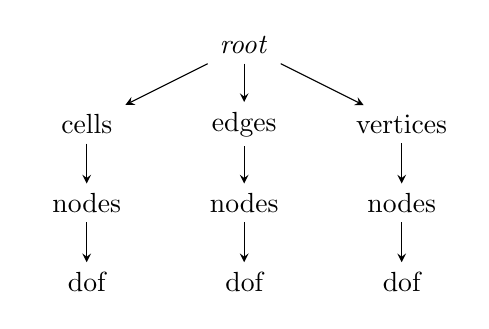
\begin{tikzpicture}
      \tikzstyle{node} = [minimum width=1.5cm,text centered,align=center];

      \node [node] (root) at (0,0) {\textit{root}};
      \node [node] (cells) at (-2,-1) {cells};
      \node [node] (edges) at (0,-1) {edges};
      \node [node] (verts) at (2,-1) {vertices};
      \node [node] (cnodes) at (-2,-2) {nodes};
      \node [node] (enodes) at (0,-2) {nodes};
      \node [node] (vnodes) at (2,-2) {nodes};
      \node [node] (cdofs) at (-2,-3) {\glspl{dof}};
      \node [node] (edofs) at (0,-3) {\glspl{dof}};
      \node [node] (vdofs) at (2,-3) {\glspl{dof}};

      \draw [-{stealth}] (root) -- (cells);
      \draw [-{stealth}] (root) -- (edges);
      \draw [-{stealth}] (root) -- (verts);
      \draw [-{stealth}] (cells) -- (cnodes);
      \draw [-{stealth}] (edges) -- (enodes);
      \draw [-{stealth}] (verts) -- (vnodes);
      \draw [-{stealth}] (cnodes) -- (cdofs);
      \draw [-{stealth}] (enodes) -- (edofs);
      \draw [-{stealth}] (vnodes) -- (vdofs);
    \end{tikzpicture}
    \caption{Example data layout tree for a 2D \py{Dat}.}
    \label{fig:vdat_tree}
  \end{subfigure}

  \begin{subfigure}{.9\textwidth}
    \begin{minted}[xleftmargin=4em,fontsize=\footnotesize]{python}
root = (
  MultiAxis()
  .add_part(AxisPart(ncells, id="cells"))
  .add_part(AxisPart(nedges, id="edges"))
  .add_part(AxisPart(nverts, id="verts"))
  .add_subaxis("cells", AxisPart(ncnodes, id="cnodes"))
  .add_subaxis("edges", AxisPart(nenodes, id="enodes"))
  .add_subaxis("verts", AxisPart(nvnodes, id="vnodes"))
  .add_subaxis("cnodes", AxisPart(ncdofs))
  .add_subaxis("enodes", AxisPart(nedofs))
  .add_subaxis("vnodes", AxisPart(nvdofs))
)
    \end{minted}
    \caption{\pyop3 code for constructing the tree structure shown above.}
    \label{lis:demotreecode}
  \end{subfigure}
  \caption{Example data layout.}
  \label{fig:demotree}
\end{figure}

Having constructed such a data layout, we address it via the use of a \textit{typed multi-index}.
This is an object of the form $\big[(t_1, i_1), (t_2, i_2), \dots, (t_n, i_n)\big]$ where $t_x$ (the `type') indicates the correct \py{AxisPart} to use in the hierarchy.
To streamline the notation, each multi-index entry in the remainder of the report will be written in the form $\mathit{type}_{\mathit{index}}$ (e.g. $c_0$ might indicate the type as `cells' with index 0).

For each \py{AxisPart}, and given an index into it ($i_x$), we use \textit{layout functions} to determine its location in memory and these offsets are added together to get the final address.
A layout function is a function that takes in an index and returns an offset.
In the case of axes with constant stride this simply takes the form \py{off = iX * stride}, but for non-constant strides it would resemble \py{off = offsets[iX]}.

The process of actually determining the address of a particular multi-index simply requires a \textit{pre-order tree visitor} algorithm to traverse the tree and accumulate the outputs of the layout functions at each level, before dispatching to the right child depending upon the `type' argument of the multi-index.

One major challenge presented by this new layout is that axes are no longer homogeneous.
In Figure~\ref{fig:vdat_pyop3} for instance, not all points have the same number of nodes per point.
This means that one can no longer stride over the axis by a constant value, and instead a lookup table must be used.

% TODO: This bit should probably be moved/broken up
This approach is advantageous because it is much more natural to reason about mesh operations at the level of mesh points.
DMPlex restrictions naturally map points to points instead of points to nodes, making map composition tractable.
The approach also facilitates: `mixed' data structures, orienting \glspl{dof} (Section~\ref{sec:impl_orientation}), data layout optimisations (Section~\ref{sec:impl_datalayoutopt}), and extruded and other partially-structured meshes (Section~\ref{sec:future_partialstructure}).

\subsubsection{Maps}
\label{sec:impl_datalayout_maps}

When we address some data, the provided data structure is associated with a particular multi-index.
When we directly address data structures, for example by doing the following:

\begin{minted}[xleftmargin=4em]{python}
loop(c := mesh.cells.index, kernel(dat0[c]))
\end{minted}

Then the multi-index getting used, \py{c}, is simply $[(C, i)]$.
This is a multi-index with only a single entry which targets all entries in the selected \py{AxisPart}, in this case all cells in the mesh.
We remark that only the outermost axes need be indexed - the inner axes (here nodes-per-cell and \glspl{dof}-per-node) are automatically included as full slices.

Since computing stencils requires the addressing of adjacent mesh points, we use \textit{maps} to describe which multi-indexes are required.
To make things clear, a map is defined as a \textit{function that accepts a multi-index and returns multiple multi-indexes}:

\vspace{1em}
\begin{equation*}
  ((t_1, i_1),) \to ((u^1_1, j^1_1),) ,\ ((u^2_1, j^2_1),) ,\ \dots ,\ ((u^m_1, j^m_1),).
\end{equation*}
\vspace{1em}

As an example, assuming a triangular mesh, the code

\begin{minted}[xleftmargin=4em]{python}
loop(c := mesh.cells.index, kernel(dat[closure(c)]))
\end{minted}

uses the $\closure$ DMPlex restriction operation to yield a map of the form

\vspace{1em}
\begin{equation*}
  ((C, c_0),)
  \to ((C, c_0),)
  ,\ ((E, e_0),) ,\ ((E, e_1),) ,\ ((E, e_2),)
  ,\ ((V, v_0),) ,\ ((V, v_1),) ,\ ((V, v_2),).
\end{equation*}
\vspace{1em}

In an analogous way to layout functions, maps can be implemented either using index functions (i.e. $e_0 = f(c_0)$), or lookup tables (\py{e0 = map[c0]}) depending on whether or not there is structure to exploit in the data layout.
This enables, for example, the use of structured meshes without needing to incur the memory bandwidth cost of tabulating a lookup table.

The approach just described enables arbitrary map composition because maps now work in line with how DMPlex handles restrictions, namely functions between mesh points, rather than between points and nodes.
One can, for example, easily describe stencils over interior facets where the stencil is composed of \textit{the closure of the cells incident on a facet}, or, in DMPlex terminology, $\closure(\support(p))$:

\begin{minted}[xleftmargin=4em]{python}
do_loop(
  f := mesh.interior_facets.index,
  kernel(
    dat0[closure(support(f))],
    dat1[closure(support(f))]
  )
)
\end{minted}

Note that at present we restrict maps to only work for multi-indices where the `parent' indices are the same for the input and output indices.
This is sufficient for unstructured meshes but not for partially-structured meshes.
This is discussed in detail in Section~\ref{sec:future_partialstructure_maps}.

\subsubsection{Raggedness and sparsity}
\label{sec:impl_datalayout_ragged}

There are occasions where one needs a data structure where the extent of an inner dimension depends on an outer one.
This occurs for example in variable layer extruded meshes - the extent of the inner dimension (the columns) is dependent upon the mesh point in the base mesh.
To get this to work, \pyop3 needs to generate code that resembles:

\begin{minted}[xleftmargin=4em]{c}
for (int i=0; i<N; ++i)
  for (int j=0; j<nlayers[i]; ++j)
    ...
\end{minted}

Note how the inner loop extent is dependent upon the outer one via the \clang{nlayers} array.

In \pyop3, such a `ragged' data structure can be initialised in the following way:

\begin{minted}[xleftmargin=4em]{python}
nlayers = Dat(MultiAxis(AxisPart(N)), dtype=int)
root = (
  MultiAxis()
  .add_part(AxisPart(N, id="outer"))
  .add_subaxis("outer", AxisPart(nlayers))
)
\end{minted}

Instead of using a constant integer value to prescribe the extent of the inner \py{AxisPart}, another \py{MultiAxis}-using data structure is used instead.
Having extents also use \py{MultiAxes} is advantageous as the code generation procedure can be shared.

We can also use the same technique to generate code for maps with \textit{variable arity}.
An example of this would be for $\plexstar(p)$ for $p$ a vertex since the number of incident edges on a vertex is variable.
This is useful for patch-based computations (see Section~\ref{sec:future_patch}).

Although not yet implemented, it should be entirely possible to implement sparse data structures by making small extensions to the existing abstraction.
If we consider a sparse matrix compressed with compressed-sparse-row (CSR) format, the data layout is described using two arrays: the row and column indices.
This is very similar to our existing solution for ragged arrays except that we assume that the internal dimension is logically dense, and hence do not need to specify column indices.

It should be noted however that we are assuming that the matrix is local to a single processor.
Parallel sparse matrices are considerably more challenging to implement and so we defer the work to PETSc (see Section~\ref{sec:impl_parallel}).

\subsubsection{Orienting degrees-of-freedom}
\label{sec:impl_orientation}

Having a hierarchical, `mesh-aware' data layout makes it much more straightforward to correctly handle orientations when packing stencils.
The way it works is as follows:
1) The DMPlex restrictions return orientation information of the mesh entities as well as the multi-index,
2) Each axis below the one selected by the map is transformed according to some predefined rule, using the orientation as a selector for the transformation.

As an example, we refer back to Figure~\ref{fig:orient_vector_flip}.
Noting that the data layout will decompose into points, nodes-per-point and \glspl{dof}-per-node, the transformation to canonical layout is done in two steps: permuting the nodes on the edge and flipping the individual \glspl{dof} such that they point in the right direction.
These operations map naturally to the different sub-axes of the data layout - the permutation applies to nodes and so can apply to the node axis, and the reflection applies to each \glspl{dof} individually and so can be applied to the \glspl{dof} axis.

\subsubsection{Data layout transformations}
\label{sec:impl_datalayoutopt}

\begin{figure}
  \centering
  \begin{subfigure}{.65\textwidth}
    \centering
    \begin{tikzpicture}[y=-1cm,scale=.75]
      \begin{scope}[xshift=3.25cm, yshift=0cm]
        \filldraw[draw=black, fill=blue!60] (0,0) rectangle (1,1);
        \filldraw[draw=black, fill=red!60] (1,0) rectangle (2,1);
        \node[at={(.5,.5)}, ptlabel] {$V_0$};
        \node[at={(1.5,.5)}, ptlabel] {$V_1$};
      \end{scope}

      \begin{scope}[yshift=-2cm]
        \begin{scope}[xshift=0cm]
          \fill[lightgray] (0,0) rectangle (4,1);
          \filldraw[draw=black, fill=white] (0.5,0) rectangle (1.5,1);
          \filldraw[draw=black, fill=white] (1.5,0) rectangle (2.5,1);
          \filldraw[draw=black, fill=white] (2.5,0) rectangle (3.5,1);
          \node[at={(1,.5)}, ptlabel] {$c_0$};
          \node[at={(2,.5)}, ptlabel] {$v_1$};
          \node[at={(3,.5)}, ptlabel] {$c_4$};
          \draw (0,0) -- (4,0);
          \draw (0,1) -- (4,1);
        \end{scope}

        \begin{scope}[xshift=4.5cm]
          \fill[lightgray] (0,0) rectangle (4,1);
          \filldraw[draw=black, fill=white] (0.5,0) rectangle (1.5,1);
          \filldraw[draw=black, fill=white] (1.5,0) rectangle (2.5,1);
          \filldraw[draw=black, fill=white] (2.5,0) rectangle (3.5,1);
          \node[at={(1,.5)}, ptlabel] {$c_0$};
          \node[at={(2,.5)}, ptlabel] {$v_1$};
          \node[at={(3,.5)}, ptlabel] {$c_4$};
          \draw (0,0) -- (4,0);
          \draw (0,1) -- (4,1);
        \end{scope}
      \end{scope}

      \draw (3.25,1) -- (0,2);
      \draw (4.25,1) -- (4,2);
      \draw (4.25,1) -- ({0+4.5},2);
      \draw (5.25,1) -- ({4+4.5},2);
    \end{tikzpicture}
    \caption{}
    \label{fig:mixedreorder_outer}
  \end{subfigure}
  %
  \begin{subfigure}{.3\textwidth}
    \centering
    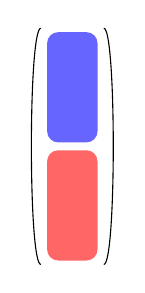
\begin{tikzpicture}[x=.8cm,y=-1cm]
      \draw (0,0) .. controls (-.2,0) and (-.2,3) .. (0,3);
      \draw (1,0) .. controls (1.2,0) and (1.2,3) .. (1,3);
      \filldraw [fill=blue!60,rounded corners,draw=none]
        (.1,.05) -- (.9,.05) -- (.9,1.45) -- (.1,1.45) -- cycle;
      \filldraw [fill=red!60,rounded corners,draw=none]
        (.1,1.55) -- (.9,1.55) -- (.9,2.95) -- (.1,2.95) -- cycle;
    \end{tikzpicture}
    \caption{}
    \label{fig:mixedreorder_outer_vec}
  \end{subfigure}

  \vspace{1em}
 
  \begin{subfigure}{.65\textwidth}
    \centering
    \begin{tikzpicture}[y=-1cm,scale=.75]
      \begin{scope}[xshift=0cm,yshift=0cm]
        \fill[lightgray] (0,0) rectangle (4,1);
        \filldraw[draw=black, fill=white] (0.5,0) rectangle (1.5,1);
        \filldraw[draw=black, fill=white] (1.5,0) rectangle (2.5,1);
        \filldraw[draw=black, fill=white] (2.5,0) rectangle (3.5,1);
        \node[at={(1,.5)}, ptlabel] {$c_0$};
        \node[at={(2,.5)}, ptlabel] {$v_1$};
        \node[at={(3,.5)}, ptlabel] {$c_4$};
        \draw (0,0) -- (4,0);
        \draw (0,1) -- (4,1);
      \end{scope}

      \begin{scope}[xshift=1cm, yshift=-2cm]
        \filldraw[draw=black, fill=blue!60] (0,0) rectangle (1,1);
        \filldraw[draw=black, fill=red!60] (1,0) rectangle (2,1);
        \node[at={(.5,.5)}, ptlabel] {$V_0$};
        \node[at={(1.5,.5)}, ptlabel] {$V_1$};
      \end{scope}

      \draw (1.5,1) -- (1,2);
      \draw (2.5,1) -- (3,2);
    \end{tikzpicture}
    \caption{}
    \label{fig:mixedreorder_inner}
  \end{subfigure}
  %
  \begin{subfigure}{.3\textwidth}
    \centering
    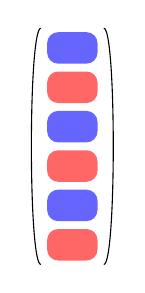
\begin{tikzpicture}[x=.8cm,y=-1cm]
      \tikzstyle{entry} = [rounded corners,draw=none];
      \tikzstyle{blue} = [entry,blue!60];
      \tikzstyle{red} = [entry,red!60];
      \draw (0,0) .. controls (-.2,0) and (-.2,3) .. (0,3);
      \draw (1,0) .. controls (1.2,0) and (1.2,3) .. (1,3);
      \filldraw [blue] (.1,.05) -- (.9,.05) -- (.9,.45) -- (.1,.45) -- cycle;
      \filldraw [red] (.1,.55) -- (.9,.55) -- (.9,.95) -- (.1,.95) -- cycle;
      \filldraw [blue] (.1,1.05) -- (.9,1.05) -- (.9,1.45) -- (.1,1.45) -- cycle;
      \filldraw [red] (.1,1.55) -- (.9,1.55) -- (.9,1.95) -- (.1,1.95) -- cycle;
      \filldraw [blue] (.1,2.05) -- (.9,2.05) -- (.9,2.45) -- (.1,2.45) -- cycle;
      \filldraw [red] (.1,2.55) -- (.9,2.55) -- (.9,2.95) -- (.1,2.95) -- cycle;
    \end{tikzpicture}
    \caption{}
    \label{fig:mixedreorder_inner_vec}
  \end{subfigure}
  \caption{}
  \label{fig:mixedreorder}
\end{figure}


With this decomposition of data layouts in a flexible, declarative hierarchy, it is now relatively straightforward to reason about making \textit{data layout transformations} to improve properties such as the effective working-set size (Section~\ref{sec:background_opt_locality}).

Some of the possible optimisations include:

\begin{paragraph}{Swapping axes}
\pyop3 makes it straightforward to swap a pair of \py{MultiAxis} such that the `inner' axis becomes the `outer' and vice versa.

An example of this is shown in Figure~\ref{fig:mixedreorder}.
Typically a `mixed' system like this - here formed of $V_0$ and $V_1$ - stores data in a blocked format (Figures~\ref{fig:mixedreorder_outer} and~\ref{fig:mixedreorder_outer_vec}).
This means that the \glspl{dof} corresponding to the same mesh point for $V_0$ and $V_1$ are very far apart in memory.
If they are both used in the local computation then this constitutes poor data locality.

To rectify the situation, we can, when applicable, permute the axes such that the mixed components are stored per mesh point, adjacent in memory.
An example of this is shown in Figures~\ref{fig:mixedreorder_inner} and~\ref{fig:mixedreorder_inner_vec}.
\end{paragraph}

\begin{paragraph}{Reordering data within axes}
Once the axes have been ordered in the most advantageous way, we can now begin to rearrange the entries in a \py{MultiAxis} to maximise locality.
In the context of meshes, these reorderings could correspond to, for example, an \gls{rcm} renumbering of the mesh entities or a different ordering of the elements up the columns of an extruded mesh.
In addition to improving locality, one can also perform these reorderings in order to allow for efficient subset queries.
Certain preconditioners require access to subsets of the mesh entities and the data layout can be modified so that the relevant \glspl{dof} are contiguous in memory.

To implement this reordering, \pyop3 simply requires that a different layout function be given to the respective \py{AxisParts}.
\end{paragraph}

\subsubsection{Other locality optimisations}

\pyop3's abstraction also enables code transformations such as vectorisation and tiling (Section~\ref{sec:background_opt_locality}).
Such optimisations are not data layout transformations, but transformations of the iteration set (i.e. the multi-index).
In both cases, the flat iteration over some axis needs to be transformed to a set of nested loops of the form

\begin{minipage}{\textwidth}
\begin{minted}[xleftmargin=4em]{c}
for (int i=0; i<NOUTER; ++i) {
  for (int j=0; j<NINNER; ++j) {
    int k = i*NINNER + j;
    ...
  }
}
\end{minted}
\end{minipage}

In the case of vectorisation, \clang{NINNER} would correspond to the length of the vector lanes of the CPU, and if tiling it would be tailored to its cache sizes.

It is valuable to note that, for unstructured meshes, tiling on its own is redundant as the amount of data shared between successive loops and prefetched by the hardware is already maximised by having an appropriate mesh numbering.
The optimisation only becomes valuable when combined with kernel fusion to produce time tiling.
Then the size of tiles should be chosen such that data required for both loops remains in cache between kernel invocations.

\subsubsection{Enabling new research}

In addition to the performance benefits espoused above, this new data layout abstraction should enable one to implement a number of new mathematical methods heretofore impossible to implement in \pyop2:

\begin{itemize}
  \item
    \textbf{p-adaptivity}
    In order to reduce the errors in a simulation, one may vary the polynomial degree of particular cells in a process known as p-adaptivity.
    It is tricky to automate a stencil code for looping over the mesh because:
    a) multiple local kernels are needed, one for each degree, and b) there are `hanging' \glspl{dof} at the boundaries between cells of differing degrees.
    Problem (a) is trivial to resolve in \pyop3.
    Rather than having a \py{MultiAxis} that is composed only of cells, edges and vertices (each a distinct \py{AxisPart}), additional \py{AxisParts} can be added such that mesh points of different degree are associated with a unique \py{AxisPart}.
    Problem (b) is more challenging to solve and requires the addition of \textit{constraints} to the abstraction (Section~\ref{sec:future_constraints}).

  \item
    \textbf{Mixed meshes}
    A mixed mesh is a mesh composed of multiple different types of polytope (e.g. triangles and squares).
    Iterating over such a mesh poses the same fundamental problem as p-adaptivity: different local kernels are required depending on the polytope type.
    Since \pyop3 is `mesh-aware' and can reason about the different classes of mesh points, this problem becomes trivial.

  \item
    \textbf{Particle-in-cell methods}
    Particle-in-cell methods are a type of numerical method where the cells of a mesh are associated with a number of, possibly advecting, particles.
    Since the number of particles differs between cells, a variable arity map is required to address them (Section~\ref{sec:impl_datalayout_ragged}).
\end{itemize}

\subsection{Parallel design}
\label{sec:impl_parallel}

\begin{figure}
  \centering
  \begin{tikzpicture}[scale=1.3]
    % define styles
    \tkzSetUpStyle[draw=white,line width=5]{cell}
    \tkzSetUpStyle[line width=2,shorten >=.2cm,shorten <=.2cm]{edge}

    \tkzSetUpStyle[cell,fill=red!50]{p1cell}
    \tkzSetUpStyle[cell,fill=red!25]{p1cellhalo}
    \tkzSetUpStyle[edge,draw=red!80]{p1edge}
    \tkzSetUpStyle[draw=red!80,fill=red!80]{p1vert}
    \tkzSetUpStyle[cell,fill=blue!50]{p2cell}
    \tkzSetUpStyle[cell,fill=blue!25]{p2cellhalo}
    \tkzSetUpStyle[edge,draw=blue!80]{p2edge}
    \tkzSetUpStyle[draw=blue!80,fill=blue!80]{p2vert}

    \tkzSetUpStyle[densely dashed,shorten >=.1cm,shorten <=.1cm,line width=.5]{connector}

    % process 
    \begin{scope}
      % define nodes
      \tkzDefPoint(0,0){p1v0}
      \tkzDefPoint(.1,1.1){p1v1}
      \tkzDefPoint(0,1.9){p1v2}
      \tkzDefPoint(.2,3.1){p1v3}
      \tkzDefPoint(1.1,0){p1v4}
      \tkzDefPoint(1,1){p1v5}
      \tkzDefPoint(.9,2){p1v6}
      \tkzDefPoint(1,3){p1v7}
      \tkzDefPoint(2,0){p1v8}
      \tkzDefPoint(2.1,1){p1v9}
      \tkzDefPoint(2,2.1){p1v10}
      \tkzDefPoint(1.9,3.2){p1v11}
      \tkzDefPoint(3,-.1){p1v12}
      \tkzDefPoint(3.1,.9){p1v13}
      \tkzDefPoint(3,2.1){p1v14}
      \tkzDefPoint(3.1,3.1){p1v15}

      % cells
      \tkzDrawPolygon[p1cell](p1v0,p1v1,p1v4)
      \tkzDrawPolygon[p1cell](p1v1,p1v4,p1v5)
      \tkzDrawPolygon[p1cell](p1v1,p1v5,p1v6)
      \tkzDrawPolygon[p1cell](p1v1,p1v2,p1v6)
      \tkzDrawPolygon[p1cell](p1v2,p1v3,p1v6)
      \tkzDrawPolygon[p1cell](p1v3,p1v6,p1v7)
      \tkzDrawPolygon[p1cell](p1v4,p1v8,p1v9)
      \tkzDrawPolygon[p1cell](p1v4,p1v5,p1v9)
      \tkzDrawPolygon[p1cell](p1v5,p1v9,p1v10)
      \tkzDrawPolygon[p1cell](p1v5,p1v6,p1v10)
      \tkzDrawPolygon[p1cell](p1v6,p1v7,p1v10)
      \tkzDrawPolygon[p1cell](p1v7,p1v10,p1v11)
      \tkzDrawPolygon[p1cell](p1v8,p1v9,p1v12)
      \tkzDrawPolygon[p2cellhalo](p1v9,p1v12,p1v13)
      \tkzDrawPolygon[p2cellhalo](p1v9,p1v13,p1v14)
      \tkzDrawPolygon[p1cell](p1v9,p1v10,p1v14)
      \tkzDrawPolygon[p2cellhalo](p1v10,p1v14,p1v15)
      \tkzDrawPolygon[p1cell](p1v10,p1v11,p1v15)

      % edges
      \tkzDrawSegments[p1edge](p1v4,p1v5 p1v5,p1v6 p1v6,p1v7)
      \tkzDrawSegments[p1edge](p1v8,p1v9 p1v9,p1v10 p1v10,p1v11)
      \tkzDrawSegments[p2edge,opacity=.5](p1v12,p1v13 p1v13,p1v14 p1v14,p1v15)

      \tkzDrawSegments[p1edge](p1v0,p1v4 p1v4,p1v8)
      \tkzDrawSegments[p1edge](p1v1,p1v5 p1v5,p1v9)
      \tkzDrawSegments[p1edge](p1v2,p1v6 p1v6,p1v10)
      \tkzDrawSegments[p1edge](p1v3,p1v7 p1v7,p1v11 p1v11,p1v15)
      \tkzDrawSegments[p2edge,opacity=.5](p1v8,p1v12 p1v9,p1v13 p1v10,p1v14)

      \tkzDrawSegments[p1edge](p1v1,p1v4 p1v1,p1v6 p1v3,p1v6)
      \tkzDrawSegments[p1edge](p1v4,p1v9 p1v5,p1v10 p1v7,p1v10)
      \tkzDrawSegments[p2edge,opacity=.5](p1v9,p1v12 p1v9,p1v14 p1v10,p1v15)  % mimics process 2

      % vertices
      % \tkzDrawPoints[p1vert](p1v0,p1v1,p1v2,p1v3,p1v4,p1v5,p1v6,p1v7)  % core
      \tkzDrawPoints[p1vert,size=5](p1v4,p1v5,p1v6,p1v7)  % core
      % \tkzDrawPoints[p1vert,diamond,size=6](p1v8,p1v9,p1v10,p1v11)  % owned
      \tkzDrawPoints[p1vert,diamond,size=6](p1v8,p1v9,p1v11)  % owned
      \tkzDrawPoints[p1vert,diamond,size=6,draw=black](p1v10)  % owned
      \tkzDrawPoints[p2vert,diamond,opacity=.5,size=6](p1v12,p1v13,p1v14,p1v15)

      % debugging
      % \tkzLabelPoints[anchor=south,font=\tiny](p1v0,p1v1,p1v2,p1v3,p1v4,p1v5,p1v6,p1v7,p1v8,p1v9,p1v10,p1v11,p1v12,p1v13,p1v14,p1v15)

      % draw a sample patch
      \tkzDefShiftPoint[p1v7](-.2,.2){p1v7patch}
      \tkzDefShiftPoint[p1v11](0,.2){p1v11patch}
      \tkzDefShiftPoint[p1v15](.2,.2){p1v15patch}
      \tkzDefShiftPoint[p1v14](.2,-.1){p1v14patch}
      \tkzDefShiftPoint[p1v9](.1,-.2){p1v9patch}
      \tkzDefShiftPoint[p1v5](-.2,-.2){p1v5patch}
      \tkzDefShiftPoint[p1v6](-.2,0){p1v6patch}
      \filldraw[draw=black,fill=black,fill opacity=.1,rounded corners=3]
      % \filldraw[draw=none,fill=blue,fill opacity=.4,rounded corners=2]
      % \filldraw[pattern={Hatch[distance=3mm,angle=45]},draw=black,rounded corners=2]
        (p1v7patch) -- (p1v11patch) -- (p1v15patch) -- (p1v14patch) -- (p1v9patch) --
        (p1v5patch) -- (p1v6patch) -- cycle;
      % \draw (p1v10) circle [radius=5pt];
      % \tkzDrawPoint[size=1pt](p1v10)

      % label "core" and "owned"
      \node (p1core) [inner sep=0pt,xshift=-20pt,yshift=20pt] at (p1v7) {\footnotesize core};
      \node (p1owned) [inner sep=0pt,xshift=-10pt,yshift=20pt] at (p1v11) {\footnotesize owned};
      \draw [-{stealth},shorten >=4pt,shorten <=2pt] (p1core.south) -- (p1v7.north);
      \draw [-{stealth},shorten >=4pt,shorten <=2pt] (p1owned.south) -- (p1v11.north);
    \end{scope}

    % process 2
    \begin{scope}[xshift=5cm]
      % define nodes
      \tkzDefPoint(0,0){p2v0}
      \tkzDefPoint(.1,1){p2v1}
      \tkzDefPoint(0,2.1){p2v2}
      \tkzDefPoint(-.1,3.2){p2v3}
      \tkzDefPoint(1,-.1){p2v4}
      \tkzDefPoint(1.1,.9){p2v5}
      \tkzDefPoint(1,2.1){p2v6}
      \tkzDefPoint(1.1,3.1){p2v7}
      \tkzDefPoint(2,-.1){p2v8}
      \tkzDefPoint(2,1.1){p2v9}
      \tkzDefPoint(2.1,2){p2v10}
      \tkzDefPoint(2,2.9){p2v11}
      \tkzDefPoint(3,.1){p2v12}
      \tkzDefPoint(3.1,1){p2v13}
      \tkzDefPoint(2.9,2){p2v14}
      \tkzDefPoint(2.9,3.1){p2v15}

      % cells
      \tkzDrawPolygon[p1cellhalo](p2v0,p2v1,p2v4)
      \tkzDrawPolygon[p2cell](p2v1,p2v4,p2v5)
      \tkzDrawPolygon[p2cell](p2v1,p2v5,p2v6)
      \tkzDrawPolygon[p1cellhalo](p2v1,p2v2,p2v6)
      \tkzDrawPolygon[p2cell](p2v2,p2v6,p2v7)
      \tkzDrawPolygon[p1cellhalo](p2v2,p2v3,p2v7)
      \tkzDrawPolygon[p2cell](p2v4,p2v5,p2v8)
      \tkzDrawPolygon[p2cell](p2v5,p2v8,p2v9)
      \tkzDrawPolygon[p2cell](p2v5,p2v6,p2v9)
      \tkzDrawPolygon[p2cell](p2v6,p2v9,p2v10)
      \tkzDrawPolygon[p2cell](p2v6,p2v10,p2v11)
      \tkzDrawPolygon[p2cell](p2v6,p2v7,p2v11)
      \tkzDrawPolygon[p2cell](p2v8,p2v9,p2v12)
      \tkzDrawPolygon[p2cell](p2v9,p2v12,p2v13)
      \tkzDrawPolygon[p2cell](p2v9,p2v10,p2v13)
      \tkzDrawPolygon[p2cell](p2v10,p2v13,p2v14)
      \tkzDrawPolygon[p2cell](p2v10,p2v14,p2v15)
      \tkzDrawPolygon[p2cell](p2v10,p2v11,p2v15)

      % edges
      \tkzDrawSegments[p1edge,opacity=.5](p2v0,p2v1 p2v1,p2v2 p2v2,p2v3)
      \tkzDrawSegments[p2edge](p2v4,p2v5 p2v5,p2v6 p2v6,p2v7)
      \tkzDrawSegments[p2edge](p2v8,p2v9 p2v9,p2v10 p2v10,p2v11)

      \tkzDrawSegments[p2edge](p2v0,p2v4 p2v4,p2v8 p2v8,p2v12)
      \tkzDrawSegments[p2edge](p2v1,p2v5 p2v5,p2v9 p2v9,p2v13)
      \tkzDrawSegments[p2edge](p2v2,p2v6 p2v6,p2v10 p2v10,p2v14)
      \tkzDrawSegments[p2edge](p2v7,p2v11 p2v11,p2v15)
      \tkzDrawSegments[p1edge,opacity=.5](p2v3,p2v7)

      \tkzDrawSegments[p2edge](p2v1,p2v4 p2v1,p2v6 p2v2,p2v7)
      \tkzDrawSegments[p2edge](p2v5,p2v8)
      \tkzDrawSegments[p2edge](p2v6,p2v9)
      \tkzDrawSegments[p2edge](p2v6,p2v11)
      \tkzDrawSegments[p2edge](p2v9,p2v12 p2v10,p2v13 p2v10,p2v15)

      % vertices
      \tkzDrawPoints[p2vert,size=5](p2v8,p2v9,p2v10,p2v11)  % core
      \tkzDrawPoints[p2vert,diamond,size=6](p2v4,p2v5,p2v6,p2v7)  % owned
      \tkzDrawPoints[p1vert,diamond,size=6,opacity=.5](p2v0,p2v1,p2v2,p2v3)  % halo

      % label "core" and "owned"
      \node (p2core) [inner sep=0pt,xshift=15pt,yshift=20pt] at (p2v11) {\footnotesize core};
      \node (p2owned) [inner sep=0pt,xshift=10pt,yshift=20pt] at (p2v7) {\footnotesize owned};
      \draw [-{stealth},shorten >=4pt,shorten <=2pt] (p2core.south) -- (p2v11.north);
      \draw [-{stealth},shorten >=4pt,shorten <=2pt] (p2owned.south) -- (p2v7.north);

      % debugging
      % \tkzLabelPoints[anchor=south,font=\tiny](p2v0,p2v1,p2v2,p2v3,p2v4,p2v5,p2v6,p2v7,p2v8,p2v9,p2v10,p2v11,p2v12,p2v13,p2v14,p2v15)
    \end{scope}

    % connect (sample of) equivalent points
    \draw [-{stealth},connector,shorten >=4pt,shorten <=4pt] (p1v11) to [bend left=45] (p2v3);
    \draw [{stealth}-,connector,shorten >=4pt,shorten <=4pt] (p1v15) to [bend left=45] (p2v7);
    \draw [-{stealth},connector,shorten >=4pt,shorten <=4pt] (p1v8) to [bend right=45] (p2v0);
    \draw [{stealth}-,connector,shorten >=4pt,shorten <=4pt] (p1v12) to [bend right=45] (p2v4);

    % label processes
    \node (p1name) at (1.5,4.2) {Process 1};
    \node (p2name) at (6.5,4.2) {Process 2};
  \end{tikzpicture}
  \caption{
    An example mesh distributed between two processes (red and blue).
    The mesh is intended for vertex patches (shaded) and so the overlap is chosen such that all required \glspl{dof} are stored locally.
    `Core' vertices are stored as circles and `owned' as diamonds.
    The direction of halo exchanges is indicated by the arrows.
  }
  \label{fig:halos}
\end{figure}

% same fundamental data types

% how to do insertion into off-diagonal parts in PETSc? how would that work with my stuff?

%\pyop3 has the same parallel design as \pyop2.
% ghost/halo values for overlaps
% globals with reductions
% can do variable halo size to replace exchanges with redundant communication - used in sparse tiling
% clever layout means we can exchange core, then owned, interleaving communication
% PETSc Mat for parallel matrices

% we assume ragged only works in serial

% PETSc is scalable (cite?)
% PyOP2 (via Firedrake assembly) has good weak scalability

% mention strong scaling

\subsection{Avoiding Python overhead}
\label{sec:impl_overhead}

Python is the language of choice for \pyop3 for a number of compelling reasons.
Dynamic typing and being interpreted instead of compiled makes it very fast for users to prototype code.
It also has great syntax, especially for domain-specific languages.
User scripts are frequently shorter than 100 lines of code.

The primary complaint levelled at Python is that it is much slower, often by a factor of 100, than a compiled language like C or Fortran.
In general this issue is not important in code generation frameworks like \pyop3 and Firedrake since the performance critical parts of the code - the `hot loops' - are actually compiled C code and just as fast as code that is written by hand.
The fact that the rest of the library is written in Python does not matter as only a tiny fraction of the programs runtime is spent there.

However, there is one significant occasion where this claim falls down, and our choice of Python as language causes trouble: in the strong-scaling limit (Section~\ref{sec:background_perf_efficiency}).
In this limit the problem occupying the `hot loops' is `small' and hence completes very quickly.
This means that more time is spent in the Python interpreter which is slow.
Firedrake has been observed to have poor strong-scaling behaviour~\cite{changComparativeStudyFinite2018}\footnote{The results shown in this paper are exaggerated. We found that it was possible to substantially improve scaling performance with a few minor code modifications.}.

The solution to this issue is simple: spend less time in the Python layer.
This can be accomplished in two ways: write the new hot loops in a compiled language, possibly via code generation, or avoid doing extra work in Python by applying judicious caching.
Doing the former is somewhat trivial and will not be discussed here.
We will instead focus on achieving performant caching solutions in \pyop3.

Since the principle object in \pyop3 is the loop expression, we will only discuss this.
As mentioned in Section~\ref{sec:impl_jit}, one way to execute a loop expression is to use the function \py{do_loop(...)}.
This instantiates a new loop expression and then executes it.
While concise, this function is not suitable if one wants to execute an identical loop expression repeatedly because, at each iteration, the expression needs to be hashed prior to being able to use any internal caching (e.g. for the generated code).

To resolve this particular issue one can create a persistent loop expression via the command \py{expr = loop(...)} (taking the same arguments as \py{do_loop(...)}), which can then be executed with \py{expr.apply()}.
Having a persistent expression means that it can be hashed once and any cached objects may be directly accessed.

At this point, however, care needs to be taken with the data structures involved.
The loop expression is created using `heavy' data-carrying objects like \py{Dats} and \py{Mats} and so indiscriminate caching of the expression would result in a memory leak.
Along similar lines, it is also difficult to `swap out' data structures in the loop expression without requiring the instantiation of a brand new expression.
In other words, if one wanted to, say, execute the same loop expression but write the output to a different data structure, then this would require the creation of a new loop expression and reincur the, totally unnecessary, cost of hashing the expression.

To resolve this, \pyop3 loop expressions will store \textit{weak references} to the data structures in the loop expression and \py{expr.apply} will take optional keyword arguments to swap out the data structures as appropriate (e.g. \py{expr.apply(out=mynewdat)}).
In Python, weak references are references to objects that do not increase their \textit{reference count}.
This prevents memory leaks because the lifetime of a data structure will only be tied to its own scope, they will still be cleaned up even if they are referenced in a cached loop expression.
